\section{Base-Stock Model}
\label{sec:base-stock-model}

\Opensolutionfile{ans}


The news-vendor model of Section~\ref{sec:newsvendor-models} is a suitable model to analyze an inventory system in which items are kept for one, two, or some other finite amount of time periods. In many cases, however, the assumption of a finite number of periods is a bit unnatural; think, for instance, about selling rice in a supermarket. In such cases it is more suitable to model time as infinite, and assume that the buying and selling price of times is constant over time and items never have to salvaged. When we keep the property of the inventory control policy to \emph{order up to some threshold}, we say that the inventory is under a \emph{base-stock policy}. In this section we analyze the consequences on inventory and backlogging cost for such base-stock policies. 

We first develop a set of formulas to construct, hence simulate, an inventory system in  discrete time under a  base-stock policy. The we discuss a mathematical model by which we can compute some of relevant the performance measures in a fast way..

\begin{comment}
We need to discuss the point of fixed or dynamic order quantities, and fixed versus dynamic order times in the intro of the basestock model. Like this we can position all the models. 

\begin{itemize}
\item $(T,Q)$ policy (silly policy both time and size are fixed)
\item $(T,S)$ policy (could be good fixed time variable size)
\item $(s,S)$ policy (best there is but you do not know in advance neither the time or the size. It is kind of ``nervous''.)
\end{itemize}
\end{comment}


\subsection{Simulation}

An inventory system in periodic-review and under a base-stock policy behaves as follows. Suppose the \emph{basestock} level is given by some number $r+1$. When the inventory position $\IP_i$ at end of period~$i$ is smaller than the \emph{base-stock level} $r+1$, i.e.,  when $\IP_i$ is less than or equal to the \emph{reorder level} $r$, then we issue a number of replenishment orders $R_i$ such that the inventory position becomes $r+1$ again. Thus, at the start of each period, the inventory position is equal to $r+1$. As these orders are assumed to arrive a fixed leadtime $L>0$ later, we distinguish between \emph{inventory position}  $\IP_i$ and \emph{inventory level} $\IL_i$, just as  Section~\ref{sec:variations} in which we considered the EOQ model with positive leadtime. We advise the reader to reread Exercise~\ref{ex:7}.

We write $D_i$ for the demand that arrives \emph{during} period $i$, and 
\begin{equation}\label{eq:b1}
  D[i-L, i] = \sum_{j=i-L}^i D_j
\end{equation}
for the demand that arrives during $i-L, i-L+1, \ldots, i$.   We assume that the (stochastic) demand process $\{D[i-L, i]\}$ is stationary and its distribution is given by 
\begin{align}
  \label{eq:16}
   F(x) &= \P{D[i-L, i] \leq x}.& f(x) = \P{D[i-L, i] = x}
\end{align}
The average demand during a lead time is written as
\begin{equation*}
\theta = \E{D[i-L, i]},
\end{equation*}
Note that the demand $D_i$ in period $i$ can be larger than one, due to the fact that we add up all demand that occurs between the review epochs $i-1$ and $i$.

\begin{exercise}
Check that the case with $L=0$ is also covered by~\eqref{eq:b1}. In other words, what is $D[i,i]$?
  \begin{solution}
    $D[i,i] = \sum_{j=i}^i D_j = D_i$. 
  \end{solution}
\end{exercise}


Under the base-stock policy we check the inventory position at the end of period $i$ and decide to replenish or not. Specifically,  if $\IP_i\leq r$, we order an amount 
\begin{equation}\label{eq:11}
  Q_{i+1} = (r+1 - \IP_i) \1{\IP_i \leq r}.
\end{equation}
This arrives right at the start of the period, so that if we know   the inventory position $\IP_{i-1}$ at the end of the period $i-1$, $\IP_i$ must satisfy the recursion
\begin{equation}\label{eq:10}
  \IP_{i} = \IP_{i-1}+Q_i - D_i.
\end{equation}


\begin{exercise}
  What is the reorder level $r$ for a make-to-order inventory system?

\begin{solution}
  In a make-to-order setting, there is no on-hand
  inventory. Production starts when a job comes in. Thus, if we take
  $r=-1$, then, when the inventory position hits $-1$, we issue a
  production order. Clearly, $\IL_i\leq0$ always, and $B_i$ is the number
  of jobs waiting to get served by production.
\end{solution}
\end{exercise}

\begin{exercise}
  Show 
  \begin{equation}
    \IP_{i}= \IP_0 + \sum_{j=1}^{i} (Q_j-D_j)
  \end{equation}
by using~\eqref{eq:10}.
  \begin{solution}
    \begin{align*}
    \IP_i
&= \IP_{i-1} + Q_i - D_i  \\
&= \IP_{i-2} + Q_{i-1} - D_{i-1} + Q_i - D_i  \\
&= \IP_{i-2} + Q_{i-1} +Q_i - D_{i-1} - D_i  \\
&= \IP_{i-2} + \sum_{j=i-1}^i (Q_{j} - D_{j}) \\
&= \IP_0 + \sum_{j=1}^{i} (Q_j-D_j)
    \end{align*}
  \end{solution}
\end{exercise}

\begin{exercise}
Motivate that
\begin{equation}\label{eq:9}
  \IP_{i} = r+1 - D_i
\end{equation}
\begin{solution}
From~\eqref{eq:11} it is apparent that we order an amount such that the inventory position right after placing the order is always equal to $r+1$. To get the inventory position at the end of the period, we subtract $D_i$ to get the result.
\end{solution}
\end{exercise}


\begin{exercise}
Explain that 
\begin{equation}\label{eq:22b}
Q_{i+1}=D_i.
\end{equation}
\begin{solution}
  Since each period, after ordering, starts with an inventory position $r+1$, we just need to order the demand of the previous period.
\end{solution}
\end{exercise}

Let $\IL_{i-1}$ denote the inventory level at the end of period $i-1$. Since replenishments arrive $L$ periods later, we have that
\begin{equation}\label{eq:b5}
  \IL_{i} = \IL_{i-1} + Q_{i-L} - D_i.
\end{equation}
With  this and the equations above we will work towards the very useful expression~\eqref{eq:15} in the next couple of exercises.

\begin{exercise}
Expand the above recursion~\eqref{eq:b5} to show that 
\begin{equation*}
  \IL_{i} = \IL_{i-1}+Q_{i-L-1} + Q_{i-L} - D_{i-1} - D_i.
\end{equation*}
\begin{solution}
Applying the recursion $I_{i-1}$, 
\begin{align*}
  \IL_{i} 
&= \IL_{i-1} + Q_{i-L} - D_i \\
&= (\IL_{i-1}+Q_{i-L-1} - D_{i-1}) + Q_{i-L} - D_i \\
&= \IL_{i-1}+Q_{i-L-1} + Q_{i-L} - D_{i-1} - D_i \\
\end{align*}
  \end{solution}
\end{exercise}

\begin{exercise}
  Use the previous exercise to derive
  \begin{equation}
    \IL_i= \IL_0 + \sum_{j=1}^{i-L} (Q_j-D_j) - D[i-L+1, i].
  \end{equation}
  \begin{solution}
Use recursion to see that
\begin{align*}
  \IL_{i} 
&= \IL_{i-1} + Q_{i-L} - D_i \\
&= (\IL_{i-1}+Q_{i-L-1} - D_{i-1}) + Q_{i-L} - D_i \\
&= \IL_{i-1}+Q_{i-L-1} + Q_{i-L} - D_{i-1} - D_i \\
&= \IL_{i-1}+\sum_{j=i-L-1}^{i-L} Q_{j} - \sum_{j=i-1}^i D_{j} \\
&= \IL_{0}+\sum_{j=1}^{i-L} Q_{j} - \sum_{j=1}^i D_{j} &\text{as } Q_j = 0\text{ for } j\leq 0\\
&= \IL_{0}+\sum_{j=1}^{i-L} (Q_{j}-D_j) - \sum_{j=i-L+1}^i D_{j}\\
&= \IL_{0}+\sum_{j=1}^{i-L} (Q_{j}-D_j) - D[i-L+1, i].
\end{align*}
  \end{solution}
\end{exercise}


\begin{exercise}
If $\IL_0 = \IP_0$, which is entirely reasonable to assume, combine the above to derive
\begin{align}\label{eq:15}
  \IL_i = \IP_{i-L} - D[i-l+1, i]
\end{align}
\begin{solution}
  \begin{align*}
    \IL_i
&= \IL_0 + \sum_{j=1}^{i-L} (Q_j-D_j) - \sum_{j=i-L+1}^j D_j \\
&= \IP_0 + \sum_{j=1}^{i-L} (Q_j-D_j) - \sum_{j=i-L+1}^j D_j \\
&= \IP_{i-L} - \sum_{j=i-L+1}^j D_j \\
  \end{align*}
\end{solution}
\end{exercise}

\begin{exercise}
  If the starting inventory $\IL_0=\IP_0 = r+1$, conclude that
  \begin{equation}\label{eq:b2}
    \IL_i=r+1 - D[i-L, i].
  \end{equation}
Thus, the number of \emph{outstanding} demands at the end of period $i$ equals
$D[i-L, i]$. In other words,  under the basestock policy items not on-hand must be on order. 
  \begin{solution}
\begin{align*}
  \IL_i 
&= \IP_i - D[i-l+1, i] \\
&= \IP_i + D_i - D[i-l, i] \\
&= r+1 - D[i-l, i] &\text{by~\eqref{eq:9}}.
\end{align*}
  \end{solution}
\end{exercise}



\begin{exercise}
To check~\eqref{eq:b2}, explain the result for $L=0$ and $L=1$.
  \begin{solution}
    If $L=0$, we have that $D[i-L,i] = D[i,i] = D_i$. Hence, $I_i = r+1-D_i$, and this is evident: when there is no leadtime, any demand in period $i-1$ is ordered, and received, at the start of period $i$. Hence, after the order, the on-hand inventory is $r+1$. 

In a similar way, if $L=1$, $I_i = r+1 - D_{i-1}- D_i$. To see this, note that $L=1$. Hence, the  inventory level just after the order lags behind by one period of demand, so that, consequently, just after the order, the inventory level must be $r+1-D_{i-1}$. From this we need to subtract the demand $D_i$ to get the level $I_{i}$ at the end of period $i$. x
  \end{solution}
\end{exercise}

\begin{exercise}
  As a check (many students fail to notice these aspects):
  \begin{enumerate}
  \item Which of the two (inventory level or inventory position) triggers the orders?
  \item Which of the two depends on the lead time?
  \item Is there a difference inventory position and inventory level when $L=0$?
  \end{enumerate}
  \begin{solution}
    Only $\IP$ triggers the orders and only $\IL$ depends on $L$. When $L=0$, the position and level coincide.
  \end{solution}
\end{exercise}


\begin{exercise}\label{ex:5}
Make a graph, in excel, of $\{D_i\}$, $\{\IP_i\}$ and $\{\IL_i\}$ when the basestock level $r+1=6$, the leadtime $L=3$, and the demands are given by
\begin{equation*}
  D = (1,2,3,0,4,4,2,0,1,3).
\end{equation*}
\begin{solution}
We use python to carry out the computations.
\begin{pyconsole}
D = np.array([0, 1,2,3,0,4,4,2,0,1,3]) # demand during a period
L = 3 
r = 5 

DL = np.zeros_like(D) # demand during leadtime

for t in range(L):
    DL[t] = sum(D[0:t+1])

for t in range(L, len(D)):
    DL[t] = sum(D[t-L:t+1])

DL

IP = (r+1)*np.ones_like(D) - D
IP

IL = np.zeros_like(D) # end of period inventory level
IL = r+1-DL
IL
\end{pyconsole}
% \begin{center}
%   \begin{tabular}[h]{cc}
% % This file was created by matplotlib2tikz v0.6.0.
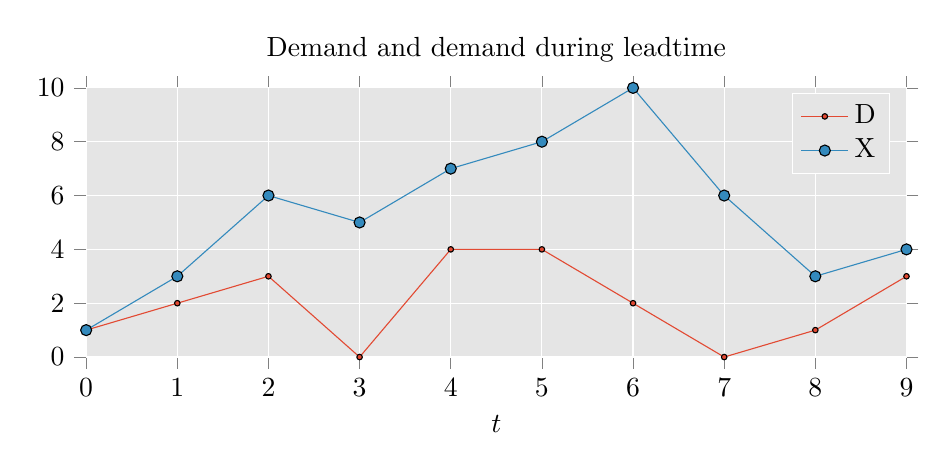
\begin{tikzpicture}

\definecolor{color0}{rgb}{0.886274509803922,0.290196078431373,0.2}
\definecolor{color1}{rgb}{0.203921568627451,0.541176470588235,0.741176470588235}

\begin{axis}[
title={Demand and demand during leadtime},
xlabel={$t$},
xmin=0, xmax=9,
ymin=0, ymax=10,
width=12cm,
height=5cm,
tick align=outside,
xmajorgrids,
x grid style={white},
ymajorgrids,
y grid style={white},
axis line style={white},
axis background/.style={fill=white!89.803921568627459!black},
legend style={draw=white, fill=white!89.803921568627459!black},
legend entries={{D},{X}},
legend cell align={left}
]
\addplot [color0, mark=*, mark size=1, mark options={solid,draw=black}]
table {%
0 1
1 2
2 3
3 0
4 4
5 4
6 2
7 0
8 1
9 3
};
\addplot [color1, mark=*, mark size=2, mark options={solid,draw=black}]
table {%
0 1
1 3
2 6
3 5
4 7
5 8
6 10
7 6
8 3
9 4
};
\end{axis}

\end{tikzpicture}\\
% % This file was created by matplotlib2tikz v0.6.0.
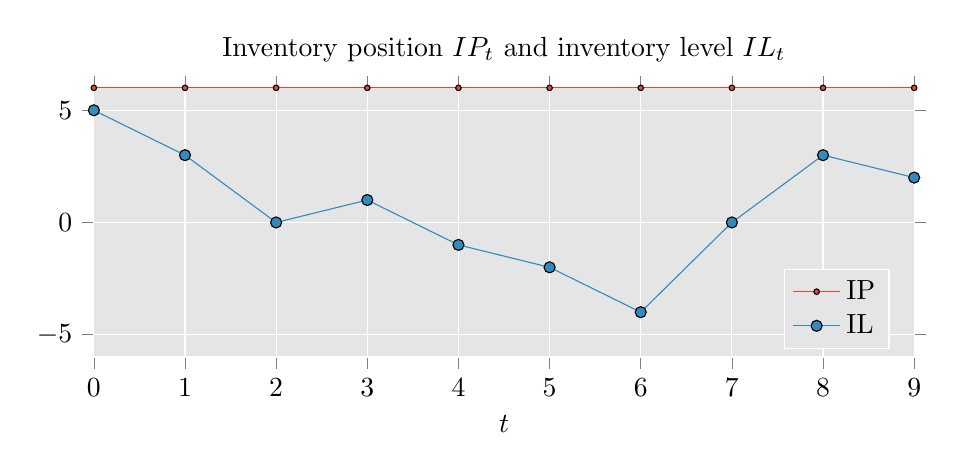
\begin{tikzpicture}

\definecolor{color0}{rgb}{0.886274509803922,0.290196078431373,0.2}
\definecolor{color1}{rgb}{0.203921568627451,0.541176470588235,0.741176470588235}

\begin{axis}[
title={Inventory position $IP_t$ and inventory level $IL_t$},
xlabel={$t$},
xmin=0, xmax=9,
ymin=-6, ymax=6,
width=12cm,
height=5cm,
tick align=outside,
xmajorgrids,
x grid style={white},
ymajorgrids,
y grid style={white},
axis line style={white},
axis background/.style={fill=white!89.803921568627459!black},
legend entries={{IP},{IL}},
legend cell align={left},
legend style={at={(0.97,0.03)}, anchor=south east, draw=white, fill=white!89.803921568627459!black}
]
\addplot [color0, mark=*, mark size=1, mark options={solid,draw=black}]
table {%
0 6
1 6
2 6
3 6
4 6
5 6
6 6
7 6
8 6
9 6
};
\addplot [color1, mark=*, mark size=2, mark options={solid,draw=black}]
table {%
0 5
1 3
2 0
3 1
4 -1
5 -2
6 -4
7 0
8 3
9 2
};
\end{axis}

\end{tikzpicture}\\
% % This file was created by matplotlib2tikz v0.6.0.
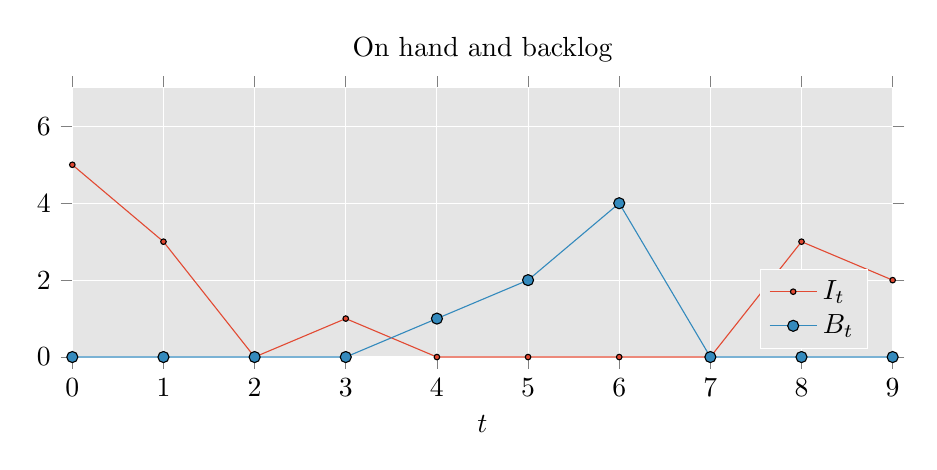
\begin{tikzpicture}

\definecolor{color0}{rgb}{0.886274509803922,0.290196078431373,0.2}
\definecolor{color1}{rgb}{0.203921568627451,0.541176470588235,0.741176470588235}

\begin{axis}[
title={On hand and backlog},
xlabel={$t$},
xmin=0, xmax=9,
ymin=0, ymax=7,
width=12cm,
height=5cm,
tick align=outside,
xmajorgrids,
x grid style={white},
ymajorgrids,
y grid style={white},
axis line style={white},
axis background/.style={fill=white!89.803921568627459!black},
legend entries={{$I_t$},{$B_t$}},
legend cell align={left},
legend style={at={(0.97,0.03)}, anchor=south east, draw=white, fill=white!89.803921568627459!black}
]
\addplot [color0, mark=*, mark size=1, mark options={solid,draw=black}]
table {%
0 5
1 3
2 0
3 1
4 0
5 0
6 0
7 0
8 3
9 2
};
\addplot [color1, mark=*, mark size=2, mark options={solid,draw=black}]
table {%
0 0
1 0
2 0
3 0
4 1
5 2
6 4
7 0
8 0
9 0
};
\end{axis}

\end{tikzpicture}
%   \end{tabular}
% \end{center}
\end{solution}
\end{exercise}




\begin{comment}
  Exercises on systems with loss
\end{comment}


\subsection{Analytic Results}

In this section we establish a set of formulas by which we can compute several performance measures as a function of the reorder level $r$. 

First, for the ready rate we have that
\begin{equation}
  \label{eq:13}
   S_r(r) = \P{\IL_i > 0} = F(r),
\end{equation}
where $F$ is defined by~\eqref{eq:16} and where we require that $i>L$ so that initial effects of the inventory no longer play a role. 


\begin{exercise}
Derive the above.
\begin{solution}
\begin{align*}
   S_r(r) &= \P{\IL_i >0} \\
   &= \P{r+1 - D[i-L, i] >0}, &\text{by \eqref{eq:b2}}  \\
   &= \P{D[i-L, i] <  r+1} \\
   & = \P{D[i-L, i] \leq  r}\\
   & = F(r)  &\text{by~\eqref{eq:16}}.
\end{align*}
\end{solution}
\end{exercise}


\begin{exercise}\label{q:basestock}
What is $S(r)$ for $r=0, \ldots, 5$ when the demand during the leadtime is given by
  \begin{align*}
    f(0) &= 1/6, & F(0) &= 1/6,  \\
    f(1) &= 1/5, & F(1)  &= 11/30,  \\
    f(2)&= 1/4, & F(2) &= 37/60, \\
    f(3) &= 1/8, & F(3)&= 89/120, \\
    f(4) &= 11/120, & F(4) &= 5/6, \\
    f(5) &= 1/6, & F(1)  &= 1.
  \end{align*}

\begin{solution}
\begin{align*}
  r &= 0 \implies S(0) = F(0) = 1/6, \\
  r &= 1 \implies S(1) = F(1) = 11/33, \\
  r &= 2 \implies S(2) = F(2) = 37/60,\\
  r &= 3 \implies S(3) = F(3) = 89/120, \\
  r &= 4 \implies S(4) = F(4) = 5/6, \\
  r &= 5 \implies S(5) = 1.
\end{align*}
\end{solution}
\end{exercise}

Next we compute the average backorder level. 

\begin{exercise}
Explain that $B_i = (D[i-L, i] - r - 1)^+$; hence a backorder only occurs  when $D[i-L, i] - r-1>0$. 
\begin{solution} Its easy to make an off-by one error. Hence, we deal with the statement in full rigor.
  \begin{align*}
    B_i 
&= I_i^- \\
&= (r+1-D[i-L, i])^- &\text{by~\eqref{eq:b2}}\\
&= (D[i-L, i]-r-1)^+.
  \end{align*}
\end{solution}
\end{exercise}

With the result of the previous exercise we can  the expected demand in backlog can be computed with the formula
  \begin{equation}  \label{eq:12}
     B(r) = \E{B_i} =\sum_{i=r+1}^\infty (i- r -1)f_i.
  \end{equation}

\begin{exercise}
Show \eqref{eq:12}. 
  \begin{solution}
\begin{align*}
     B(r) 
   &= \E{B_i} \\
   &= \E{( D[i-L, i]- r - 1)^+} \\
   &= \sum_{i=r+1}^\infty (i- r -1)\P{D[i-L, i] = i}\\
   &= \sum_{i=r+1}^\infty (i- r -1)f_i \\
   &= \sum_{i=r+2}^\infty (i- r -1)f_i,
\end{align*}
where the last equation follows from the fact that $i-r-1=0$ when $i=r+1$.
  \end{solution}
\end{exercise}

\begin{exercise}\label{q:basestock_B}
  Suppose the demand is given by  Exercise~\ref{q:basestock}. What is $B(r)$ for $r=0,\ldots, 5$.?
\begin{solution}
  Use that $B(r) = \sum_{i=r+1}^\infty (i-r-1)f(i)$, and that $f(i)=0$ for $i\geq 6$.
  \begin{align*}
    r&=0 \implies B(0) = \sum_{i=1}^\infty (i-1)f(i) =  0\cdot 1/5 + \cdots + 4 \cdot 1/6 = 173/120, \\
    r&=1 \implies B(1) = \sum_{i=2}^6 (i-2)f(i) =  1\cdot 1/8 + 2\cdot 11/120 + 3 \cdot 1/6 = 97/120, \\
    r&=2 \implies B(2) = 1\cdot 11/120 + 2 \cdot 1/6 = 17/40, \\
    r&=3 \implies B(3) = 1 \cdot 1/6 = 1/6, \\
  \end{align*}
\end{solution}
\end{exercise}

Note that in the above formula for $B(r)$ the summation runs to $\infty$, which is sometimes a bit problematic for numerical purposes. It turns out that~\eqref{eq:12} can be rewritten to 
\begin{equation} \label{eq:17}
   B(r) = \theta - \sum_{j=0}^{r} G(j)
\end{equation}
where
\begin{equation*}
    G(j) = 1 - F(j) = \P{D[i-L, i] > j},
\end{equation*}
and $\theta=\E{D[i-L, i]}$ is the average leadtime demand.

\begin{exercise}[\faRocket]
Derive~\eqref{eq:17}.
\begin{solution}
Note  that
\begin{equation*}
  \sum_{j=0}^\infty \1{j< i-r - 1} = i-r -1.
\end{equation*}
With this,
\begin{align*}
       B(r) &= 
   \sum_{i=r+1}^\infty (i-r-1) f(i)   \\
   &= \sum_{i=r+1}^\infty\sum_{j=0}^\infty \1{j < i-r-1}\, f(i)   = 
    \sum_{j=0}^\infty \sum_{i=r+1}^\infty \1{i > j +r + 1}\, f(i)\\
   &= \sum_{j=0}^\infty \sum_{i=j + r+2}^\infty  f(i) = 
   \sum_{j=0}^\infty \P{D[k-L, k] \geq j + r+2}  &\text{ for any } k \\
   &=\sum_{j=0}^\infty \P{D[k-L, k] > j + r+1} \\
   &= \sum_{j=r+1}^\infty  G(j).
\end{align*}
This can be simplified a bit further by using that
$\sum_{i=0}^\infty \bar G(i) = \theta$:
\begin{align*}
   B(r) 
   &= \sum_{j=r+1}^\infty  G(j) \\
   &= \sum_{j=0}^\infty  G(j) - \sum_{j=0}^{r} G(j)\\
   &= \theta - \sum_{j=0}^{r} G(j)
\end{align*}
\end{solution}
\end{exercise}
	   
\begin{exercise}What is $\theta$ for the demand of Exercise~\ref{q:basestock}?
\begin{solution}
  \begin{align*}
    \theta = \E{X} =
0\cdot \frac 1 6 + 1\cdot \frac 1 5 + \cdots + 5 \cdot \frac 1 6 = \frac{91}{40}.
  \end{align*}
\end{solution}
\end{exercise}

\begin{exercise}
  Show that the results of \eqref{eq:12} and \eqref{eq:17} coincide for the data of Exercise~\ref{q:basestock}.
\end{exercise}


Finally, by taking expectations at the left and right hand side of~\eqref{eq:b2} and using \eqref{eq:2a} it follows that for the average on-hand inventory 
\begin{equation}\label{eq:19}
I(r) = \E{\IL_i^+} = r+1 - \theta + B(r)
\end{equation}

\begin{exercise}
Derive \eqref{eq:19}. 
\begin{solution} We can use \eqref{eq:3} and \eqref{eq:4} to see that $\IL_i^+ - \IL_i^- = \IL_i$. Next, since $\IL_i = r+1 - D[i-L, i]$, we have that 
  \begin{equation*}
    \IL_i^+ = \IL_i + \IL_i^-=r+1 - D[i-L, i] + \IL_i^-.
  \end{equation*}
Taking expectations and recalling that $B_i = \IL_i^+$,
\begin{align*}
  \E{\IL_i^+}
  &= r+1 - \E{D[i-L, i]} + \E{B_i}  \\
  & = r + 1 - \theta + B(r).
\end{align*}
\end{solution}
\end{exercise}

\begin{exercise}
Suppose the demand is given by Exercise~\ref{q:basestock}. What is $I(r)$ for $r=0,\ldots, 5$.?

\begin{solution}
 The result follows straightaway from Exercise~\ref{q:basestock_B}. As an example
  \begin{equation*}
    I(3) = 3+1 - \theta + B(3) = 4 - 91/40 + 1/6 = 227/120.
  \end{equation*}
\end{solution}
\end{exercise}

\begin{exercise}
Suppose the demand is given by the previous exercise and that the holding cost $h=1$ and the backlog cost per item is $b=5$.  Which value for $r$ minimizes $h I(r)+b B(r)$?
\nvf{To be done}
\end{exercise}

\nvf{Do we still want to skip these formulas?} Formulas to skip (in FP edition 3): 2.24, 2.25. 

\nvf{Make the stuff for normally distributed demand, also for the q,r model?}

\Closesolutionfile{ans}
\opt{solutionfiles}{
\subsection{Solutions}
\input{ans}
}

\clearpage
%%% Local Variables:
%%% mode: latex
%%% TeX-master: "inventory_notes"
%%% End:


